
\subsubsection{DataInputStream}
\label{sec:uml:input:datainputstream}

在 Java 官方的 IO 包中,官方提供了 \lstinline|DataInputStream| 这个类。
在 API 文档中的描述如下
\begin{quote}
  A data input stream lets an application read primitive Java data types from an underlying input stream in a machine-independent way. 
  An application uses a data output stream to write data that can later be read by a data input stream.

  DataInputStream is not necessarily safe for multithreaded access. Thread safety is optional and is the responsibility of users of methods in this class.
\end{quote}

这一段描述交代了两件事, \lstinline|DataInputStream| 是一个用于读取“原始”的Java数据,并且与硬件底层无关。第二件事指出了其不是线程安全的,线程安全由用户保证。

\lstinline|DataInputStream| 继承自 \lstinline|FilterInputStream|, 同时实现了 \lstinline|DataInput| 接口。
\lstinline|DataInputStream| 的使用基本上就是以 \lstinline|DataInputStream var = new DataInputStream(new InputStream(..));| 的方式使用,类似
\lstinline|BufferedInputStream|类似。其提供了17个 read 函数的实例,分贝可以读取字节,布尔类型,字符类型,浮点类型,和整数类型,同是提供了读取一行,和跳过字节的功能。
同时还从 \lstinline|FilterInputStream| 继承了一些其他的方法。

%% 类图
如下图 \ref{fig:datainputstream} 是 这个类的 UML 类图。
\begin{figure}
\centering
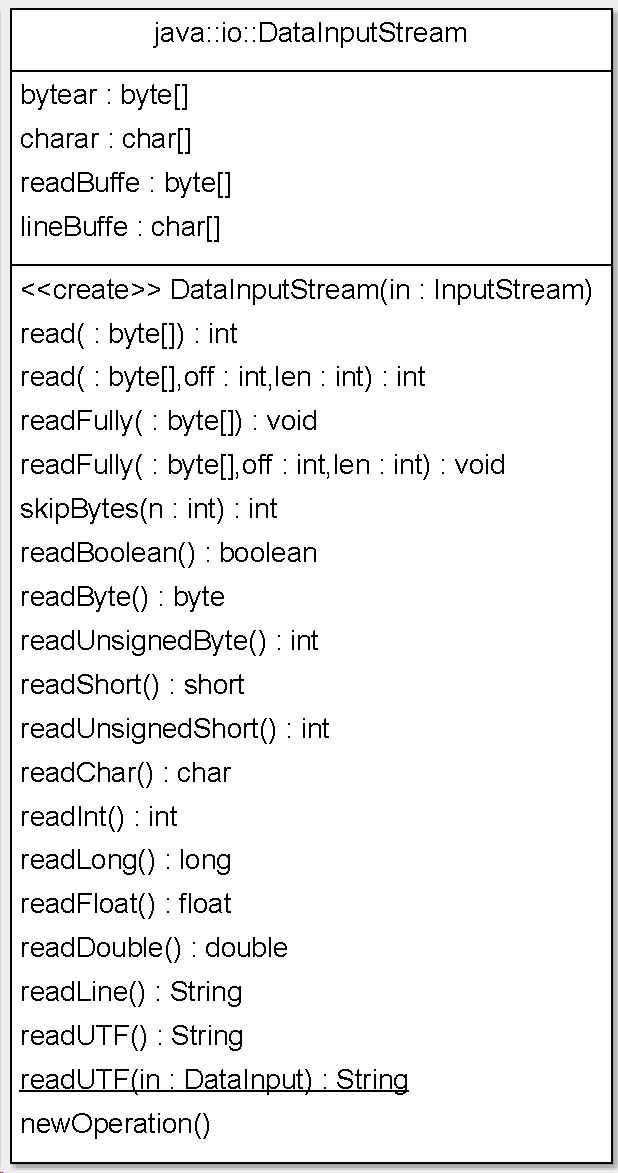
\includegraphics[width=1\linewidth]{UML/inputstream/datainputstream}
\caption{DataInputStream 类的 UML 类图}
\label{fig:datainputstream}
\end{figure}

%% 代码(主要的read)
这个类主要继承于\lstinline|FilterInputStream| 并实现了 DataInput 接口。
\begin{java}
public class DataInputStream extends FilterInputStream implements DataInput {
\end{java}
类似的,构造函数也是直接“输入” 一个\lstinline|InputStream|。
\begin{java}
    public DataInputStream(InputStream in) {
        /*...*/
    }    
\end{java}
其提供了许多读取的用的方法。有一些相对比较常见的方法,接受字节输入。 
\begin{java}
    public final int read(byte b[]) throws IOException {
        /*...*/
    }
    
    public final int read(byte b[], int off, int len) throws IOException {
        /*...*/
    }
    
    public final void readFully(byte b[]) throws IOException {
        /*...*/
    }
    
    public final void readFully(byte b[], int off, int len) throws IOException {
        /*...*/
    }
\end{java}
同时还提供了跳过字节的方法,用来跳过特定数目的字节内容。
\begin{java}
    public final int skipBytes(int n) throws IOException {
        /*...*/
    }
\end{java}
此外就是一些用于读取特定数据内容的 “read”方法。
包括读取:布尔类型,字节类型,无符号字节类型,短整型,无符号短整型,字符类型,整型,长整型,单精度浮点,双精度浮点等数据的功能。
\begin{java}    
    public final boolean readBoolean() throws IOException {
        /*...*/
    }
    
    public final byte readByte() throws IOException {
        /*...*/
    }
    
    public final int readUnsignedByte() throws IOException {
        /*...*/
    }
    
    public final short readShort() throws IOException {
        /*...*/
    }
    
    public final int readUnsignedShort() throws IOException {
        /*...*/
    }
    
    public final char readChar() throws IOException {
        /*...*/
    }
    
    public final int readInt() throws IOException {
        /*...*/
    }
    
    public final long readLong() throws IOException {
        /*...*/
    }
    
    public final float readFloat() throws IOException {
        /*...*/
    }
    
    public final double readDouble() throws IOException {
        /*...*/
    }    
\end{java}
当然也提供了读取一行喝读取 UTF 字符集字符的功能。
\begin{java}    
    @Deprecated
    public final String readLine() throws IOException {
        /*...*/
    }
    
    public final String readUTF() throws IOException {
        /*...*/
    }   
}
\end{java}
